\documentclass{sig-alternate-10pt}

\newcommand{\ttt}{\texttt}

\usepackage{graphicx}
\usepackage{changepage}
\usepackage{lipsum}
\usepackage{booktabs}

\title{FLASH\\Fast Linux Advanced Scheduler Hardware}
\author{
	Mark Aligbe \\
	    \email{ma2799@columbia.edu}
	\and
    Chae Jubb \\
        \email{ecj2122@columbia.edu}
}
\date{4 May 2015}

\begin{document}
\maketitle

\begin{abstract}
As accelerators become more common and necessary as a way to continue Moore's Law in the absence of Dennard Scaling, researchers explore segments of computation that can be improved with the aid of dedicated hardware. This paper presents FLASH, a hardware scheduler to take over the task of scheduling from the operating system. FLASH is able to make scheduling decisions in much fewer cycles as compared to modern operating system schedulers. The scheduling decisions it makes are just as good as those that would be made in software, but in much reduced time and without negatively impacting processor performance features. FLASH is designed to keep kernel modifications minimal, only requiring changes when the kernel scheduling interface changes.

\end{abstract}


\section{Introduction}
\lipsum[1-3]


\section{Scheduling in the Kernel}
% Mark
\subsection{History of Linux Schedulers}
\subsection{Implementation of CFS}
\subsection{Limitations}


\section{Related Works}
\lipsum[1-2]


\section{FLASH Architecture}
% Chae
\lipsum[1-8]


\section{Integration}
% intro stuff here
\subsection{Cyclone V}
% Mark
\begin{figure}
	\begin{center}
		%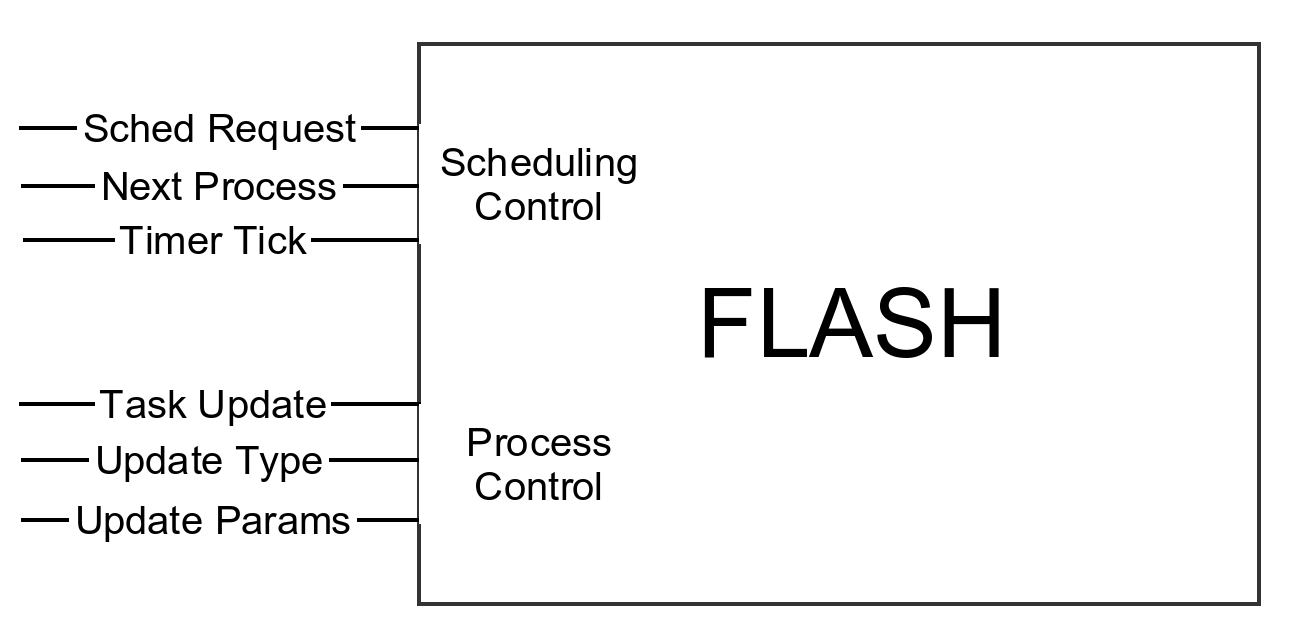
\includegraphics[width=0.65\textwidth]{fig/flash-diagram.png}
		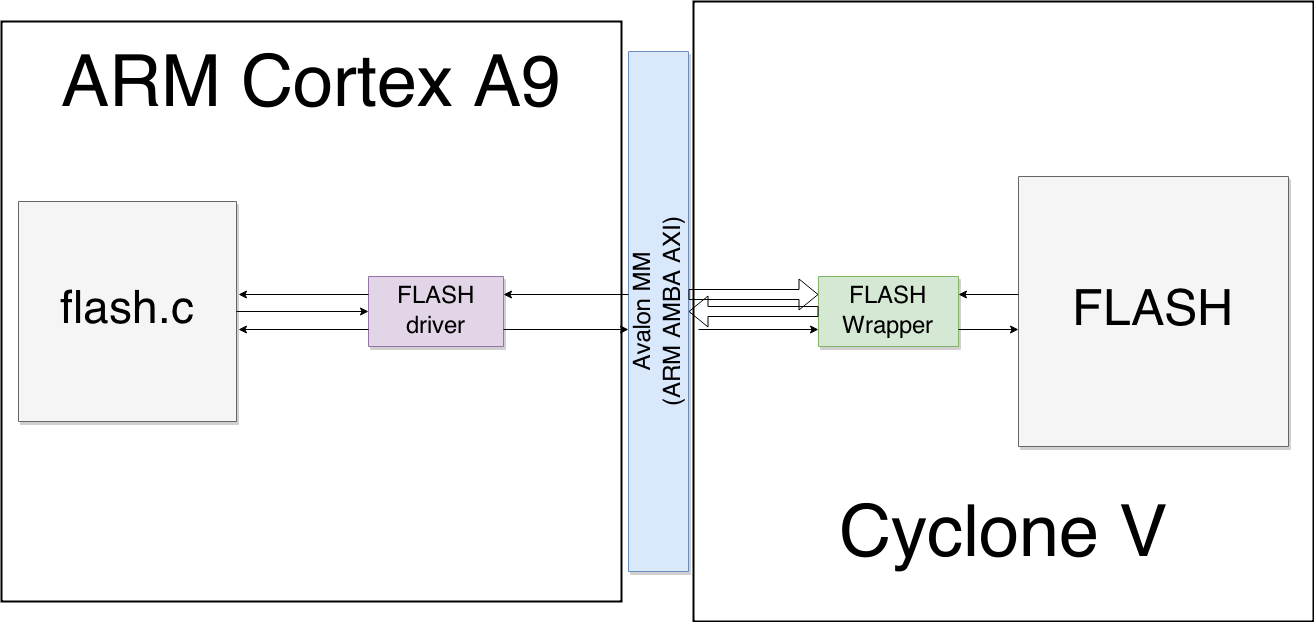
\includegraphics[width=0.9\linewidth]{fig/sockit-architecture.png}
		\caption{
			FLASH System Architecture: Interface.  Note the distinction between
			the \emph{Process Control} and \emph{Scheduling Control} Interfaces.
		}
		\label{fig:sockit_overview}
	\end{center}
\end{figure}


\subsection{Kernel mods}
% Chae
\lipsum[1-3]


\section{Applications}
% Mark
\lipsum[1-3]


\section{Engineering Experiences}
% both
\lipsum[1-3]


\section{Conclusion}
\lipsum[1]

\nocite{*}
{
	\bibliographystyle{abbrv}
	\bibliography{ref}
}

\end{document}
